% Copyright © 2013 Martin Ueding <dev@martin-ueding.de>
%
\input{header.tex}

\usepackage{tikz}
\usetikzlibrary{calc}

\newcommand{\themodul}{physik411}
\newcommand{\thegruppe}{Gruppe 2 -- Florian Seidler}
\newcommand{\theuebung}{8}

\ifoot{\footnotesize{Martin Ueding}}
\ihead{\themodul{} -- Übung \theuebung}
\ofoot{\footnotesize{\thegruppe}}

\def\thesubsection{\thesection\alph{subsection}}

\title{\themodul{} -- Übung \theuebung}
\subtitle{\thegruppe}
\author{
	Martin Ueding \footnote{\href{mailto:mu@uni-bonn.de}{mu@uni-bonn.de}}
}

\hypersetup{
	pdftitle={\themodul {} - Übung \theuebung},
}

\begin{document}

\maketitle

\begin{center}
	\ccbysadetitle
\end{center}

\begin{table}[h]
	\centering
	\begin{tabular}{l*3{|c}}
		Aufgabe
		& \ref 1
		& \ref 2
		& $\sum$   \\
		\hline
		Punkte
		& \punkte / 18
		& \punkte / 14
		& \punkte / 32
	\end{tabular}
\end{table}

%%%%%%%%%%%%%%%%%%%%%%%%%%%%%%%%%%%%%%%%%%%%%%%%%%%%%%%%%%%%%%%%%%%%%%%%%%%%%%%
%              Das Morse-Potential eines diatomischen Moleküls               %
%%%%%%%%%%%%%%%%%%%%%%%%%%%%%%%%%%%%%%%%%%%%%%%%%%%%%%%%%%%%%%%%%%%%%%%%%%%%%%%

\section{Das Morse-Potential eines diatomischen Moleküls}
\label 1

\subsection{}

\subsection{}

\subsection{Plot und Größen}

Für verschiedene $\ell$ ist das Morse-Potential in Abbildung \ref{fig:1/c/Plot}
dargestellt.

\begin{figure}
	\centering
	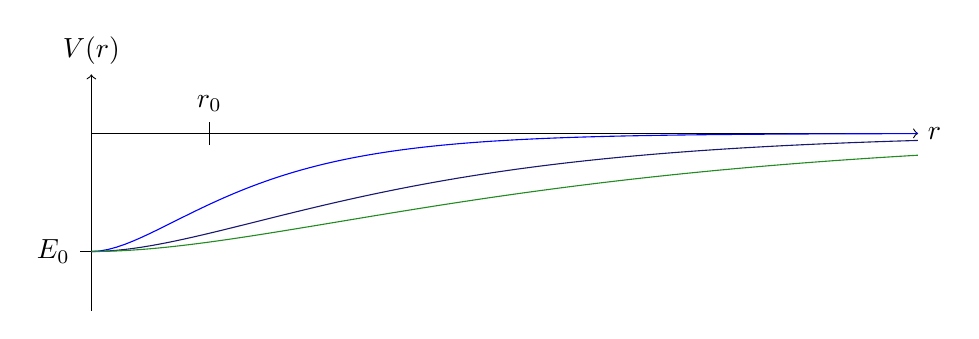
\begin{tikzpicture}[scale=1.5]
		\draw[->] (0, 0) -- ++(7, 0) node[right] {$r$};
		\draw[->] (0, -1.5) -- ++(0, 2) node[above] {$V(r)$};
		\draw (1, -.1) -- ++(0, .2) node[above] {$r_0$};
		\draw (.1, -1) -- ++(-.2, 0) node[left] {$E_0$};
		\draw[domain=0:7, samples=100, color=blue] plot (\x,{(exp(-\x) - 1)^2 - 1});
		\draw[domain=0:7, samples=100, color=MidnightBlue] plot (\x,{(exp(-\x/2) - 1)^2 - 1});
		\draw[domain=0:7, samples=100, color=ForestGreen] plot (\x,{(exp(-\x/3) - 1)^2 - 1});
	\end{tikzpicture}
	\caption{%
		In \textcolor{blue}{blau} das Morse-Potential für $\ell = 1$. In
		\textcolor{MidnightBlue}{mitternachtsblau} den Fall $\ell = 2$. Sowie
		in \textcolor{ForestGreen}{waldgrün} $\ell = 3$.
	}
	\label{fig:1/c/Plot}
\end{figure}

Die Rolle von $\ell$ scheint eine Art charakteristische Länge zu sein. Je
größer $\ell$ ist, desto länger reicht das Potential. Beim Wasserstoff ist dies
ähnlich, da die zugeordneten Laguerrefunktionen mit zunehmendem $\ell$ auch
langreichweitiger werden. Daher ist auch der Quantendefekt bei größeren $\ell$
kleiner, weil sich die Elektronen nicht mehr so häufig am Kern aufhalten.

%%%%%%%%%%%%%%%%%%%%%%%%%%%%%%%%%%%%%%%%%%%%%%%%%%%%%%%%%%%%%%%%%%%%%%%%%%%%%%%
%                                    Ende                                     %
%%%%%%%%%%%%%%%%%%%%%%%%%%%%%%%%%%%%%%%%%%%%%%%%%%%%%%%%%%%%%%%%%%%%%%%%%%%%%%%

\IfFileExists{\bibliographyfile}{
	%\bibliography{\bibliographyfile}
}{}

\end{document}

% vim: spell spelllang=de
